\documentclass[11pt,a4paper, twoside]{article}
\usepackage{polski}
\usepackage[utf8]{inputenc}
\usepackage{graphicx}
\usepackage{pdfpages}
\usepackage{minted}
\usemintedstyle{trac}
\usepackage{helvet}
\renewcommand{\familydefault}{\sfdefault}
\usepackage{sectsty}
\sectionfont{\rmfamily}
\usepackage{indentfirst}
\usepackage{hyperref}
\usepackage{subcaption}
\usepackage{graphicx}
\begin{document} 

\includepdf[pages={1,2}]{first-pages.pdf}
\tableofcontents
\newpage	
\section{Cel i zakres pracy}
Przedmiotem niniejszej pracy jest budowa mobilnego systemu pomiaru czasu dla zawodów narciarskich. System składa się z dwóch bramek: startowej oraz końcowej, które wykorzystują wiązke laserową w celu uchwicenia dokładnego momentu przejechania zawodnika przez bramkę. Niniejsza praca będzie się składać z trzech głównych części. Pierwsza z nich poświęcona zostanie architekturze systemu i wykorzystanych technologiach, a w szczególności komunikacji pomiędzy komponentami oraz podstawą teoretycznym działania. Druga część tej pracy zawiera opis implementacji, zaś trzecia część jest poświęcona umieszczeniu systemu w obudowie ochronnej.
\section{Wstęp}
Obecnie na rynku istnieją podobne systemy do tego, którego budowę ta praca przedstawia, jednak często kosztują tysiące złotych. Praca ta jest próbą stowrzenia rozwiązania spełniającego podobne zadanie do ww. systemów korzystając z ogólnie dostępnych podzespołów za nie wielkie pieniądze.

Jako szkielet systemu zostało wybrane Raspberry Pi - platforma komputerowa stworzona przez Raspberry Fundation. W momencie premiery (29 luty 2012) model B użyty w tej pracy miał cenę początkową US\$ 35. Raspberry Pi oparte jest o chip BCM2835 zawierający procesor ARM. Urządzenie działa pod kontrolą dystrybucji systemu Linux Raspbian będącą portem Debiana Wheezy (7.x) koniecznym z powodu braku kompatybilności - oficjalne wydanie Debiana Wheezy na platformę armhf jest kompatybilne jedynie z procesorami ARMv7 lub wyższymi (procesor Raspberry Pi jest procesorem ARMv6).

Obie aplikacjie (startowa i końcowa) zostały napistane przy użyciu języka Ruby 2.1.0 oraz dla aplikacji startowej stworzony został interface web umożliwiający wprowadzanie zawodników oraz podgląd wynikow, jak równiez import oraz eksport. Napisany został przy użyciu CoffeeScript oraz biblioteki JavaScript Backbone.js. 
CoffeeScript jest językiem inspirowanym elegancką składnią Ruby i Pythona, który kompiluje się do JavaScriptu. Backbone.js natomiast zapewnia strukturę aplikacji.
\newline
\newline
\noindent
W momencie pisania kodu obu aplikacji autor nie zdawał sobie jeszcze sprawy z pewnych dobrych pratyk pisania kodu, zatem w kodzie znajdują się błędy (złe praktyki), których należy unikać. Ta prace będzie się takrze pokazać na czym one polegają i jakie trudności w późniejszym utrzymaniu kodu podowują, tak aby czytelnik był ich świadom i sam ich nie popełniał.
\newline
\newline
\noindent
W pracy zostały użyte różne \em{gem-y}~-~programy i biblioteki managera paczek \emph{RubyGems}, których lista w raz z licencjami zostanie przedstawiona na końcu tej pracy.
\newline
\newline
\noindent
Kompletny kod źródłowy pracy można znaleść pod adresami:
\newline
\url{https://github.com/okapusta/skirace}
\newline
\url{https://github.com/okapusta/skirace-worker}
\section{Realizacja tematu}
\subsection{Architektura}
System, którego ta praca dotyczy został zbudowany w myśl modelu master/slave gdzie mastertem jest aplikacja początkowa. To tam znajduje się interface, baza danych oraz serwer Memcached. W momencie uruchomienia aplikacji, oprócz startu serwera serwującego aplikację WEB tworzony jest nowy wątek zawierający event-loop, który rejestruje przecięcie wiązki lasera, oraz kiedy to sie stanie ustawia godzinę tego zdarzenia w cache.

Zadaniem slavea~-~workera~-~jest jedynie pobranie czasu startu z Memcached, obliczenie czasu końcowego oraz wypisanie go na ekranie LCD linii końcowej w momencie finishu.
\newline

\begin{figure}[ht]
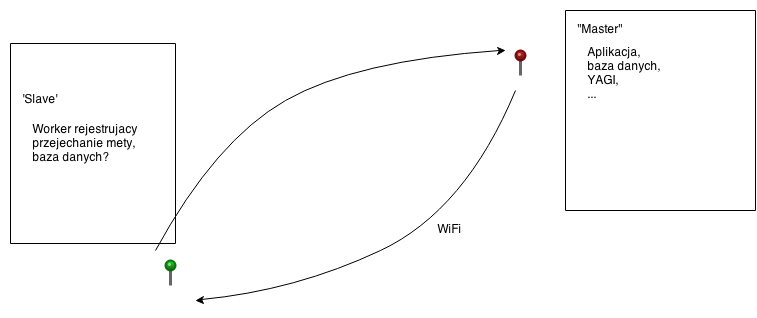
\includegraphics[scale=0.5]{./img/asdasd.png}
\end{figure}
\noindent
Komunikacjia pomiędzy dwiema bramkami odbywa się poprzez WiFi.
\paragraph{Memcached} ~\\
\newline
Memcached jest to rozproszony system buforowania pamięci podręczniej oryginalnie zaprojektowany na potrzeby serwisu  LiveJournal. Pozwala on na przechowywanie obiektów w pamięci RAM przy pomocy kluczy. W aplikacji wykorzystany został w celu przechowania czasów startu i finishu. Serwer Memcached jest uruchomiony tylko na jednej (startowej) bramce, worker natomiast łączy się z cache przy pomocy klienta i może pobierać lub pisać dane do pamięci drugiego urządzenia.
\paragraph{Dependency Injection} ~\\
\newline
W ninejszej pracy został wykorzystany wzorzec projektowy \emph{Dependency Injection (DI)} polegający na usuwaniu bespośrednich zależności klas na rzecz \emph{wstrzykiwania} ich w czasie konstruowania obiektu. Do osiągnięcia tego celu i uproszczenia  DI użyty został gem Dependor, udostępniający prosty DSL (\emph{eng. Domain Specific Language}) przeznaczony do tego celu.

Poniżej zamieszczone są listingi przedstawiające normlne wstrzykiwanie zależności w Ruby oraz z wykorzystaniem gem-u Dependor.
\newline


\begin{figure}[h]
\centering
\begin{subfigure}[t]{0.45\textwidth}
\caption{Ruby}
\begin{listing}[H]
\inputminted[linenos=true]{ruby}{./src/di_ruby.rb}
\end{listing}
\end{subfigure}
\begin{subfigure}[t]{0.45\textwidth}
\caption{Dependor}
\begin{listing}[H]
\inputminted{ruby}{./src/di_dependor.rb}
\end{listing}
\end{subfigure}
\end{figure}

\paragraph{Sprockets} ~\\
\newline
Do kompilacji CoffeeScript oraz szablonów \emph{.hamlc} (\emph{Haml Coffee Assets}) został użyty gem \emph{Sprockets} zawierający preprocessory dla języków takich jak CoffeeScript czy SCSS. Sprockets w środowisku developerskim pozwala na kompilacje assetów (JavaScriptów i CSSów) 'w locie', natomiast w środowisku produkcyjnym assety są prekompilowane. Sprockets pozwala również na minifikacje zasobów to jest zastąpienie nazw funkcji pojedyńczymi zakami w celu zmiejszenia rozmiaru kodu, który musi zostać pobrany przez przeglądarkę. 
\subsection{Implementacja}
\subsubsection{Aplikacja}
\subsubsection{Worker}
\subsection{Obudowa ochronna}
\section{Wnioski}

\end{document}